\section{第四章
编排状态机与策略分层设计}\label{ux7b2cux56dbux7ae0-ux7f16ux6392ux72b6ux6001ux673aux4e0eux7b56ux7565ux5206ux5c42ux8bbeux8ba1}

编排状态机是本框架的核心控制机制，其设计面向通用的多模块硬件设计自动化流程。状态机定义的执行阶段（规格摄入→架构设计→规划→模块设计→分层验证→集成回归→终态）适用于任何
DAG 可分解的硬件设计任务。本章先阐述状态机的通用语义设计，再以 AES-128
验证案例展示各状态的具体实例化内容。

\subsection{4.1 10
状态编排状态机}\label{ux72b6ux6001ux7f16ux6392ux72b6ux6001ux673a}

\subsubsection{4.1.1
状态定义与语义}\label{ux72b6ux6001ux5b9aux4e49ux4e0eux8bedux4e49}

本框架的编排器状态机由 \texttt{policy.py} 中的
\texttt{OrchestratorState} 枚举完整定义，共包含 10 个状态。这 10
个状态不仅是系统执行阶段的语义标记，更是 \texttt{AgentExecutionPolicy}
映射的索引键------每个状态精确决定了当前阶段应使用哪种 LLM Profile
和哪种子代理委派策略。以下逐一说明各状态的语义与行为：

\textbf{（1）SPEC\_INTAKE（规格摄入）}

规格摄入状态是整个工作流的起点，负责将设计目标解析为框架可处理的结构化规格中间表示（\texttt{SpecIR}）。该状态适用于任何硬件设计目标------框架接收设计规格，验证其是否满足自动化前提条件，并生成后续阶段所需的元数据。

在 AES-128 验证案例中，\texttt{synthesize\_spec\_ir()} 从预设的 AES-128
目标中构建 \texttt{SpecIR}
数据模型，该模型包含系统目标、算法标识符、变体（\texttt{AES-128}）、操作类型（\texttt{encrypt}）、接口风格（\texttt{block\_handshake}）、微架构（\texttt{iterative\_10\_round}）、时序目标（延迟
11 周期）及冻结接口清单。由于 \texttt{SpecIR} 带有
\texttt{@model\_validator} 约束，若目标不符合 AES MVP
范围则立即报错。这一阶段的执行主体是框架合成层，而非 LLM，故分配
\texttt{DEEPSEEK\_OFFICIAL\_THINKING} profile（用于后续若需 LLM
辅助分析规格）且子代理策略为 \texttt{FORBIDDEN}。

\textbf{（2）ARCHITECTING（架构设计）}

在架构设计状态下，\texttt{synthesize\_plan\_dag()} 从
\texttt{\_aes\_blueprints()} 蓝图生成 \texttt{PlanDAG}，包含 4
个节点及其依赖关系，并通过内置的 DFS
无环验证。该状态同样以框架合成层为主体，LLM 参与程度最低，子代理策略为
\texttt{FORBIDDEN}。

\textbf{（3）PLANNING（规划）}

规划状态负责生成
\texttt{IntegrationRegressionManifest}（集成回归清单）并初始化
\texttt{FragilityMemory}（脆弱性历史记录），为后续批调度提供必要的元数据。子代理策略为
\texttt{FORBIDDEN}。

\textbf{（4）MODULE\_DESIGN（模块设计）}

模块设计状态是 LLM
首次深度介入的状态。在此状态下，\texttt{initialize\_node\_workspace()}
为每个节点创建工作区目录结构，生成
\texttt{module\_contract.json}、\texttt{testbench\_contract.json} 和
\texttt{module\_design\_brief.json} 三份合约文件，并通过
\texttt{MemoryStore.populate\_workspace()} 将来自 Skill
文件的验证通过参考代码写入草稿 RTL 和测试台文件。工作区状态从
\texttt{MISSING} 转变为 \texttt{DRAFT\_READY}。LLM Profile 切换为
\texttt{DEEPSEEK\_OFFICIAL\_FAST}，子代理策略为
\texttt{MODULE\_WORKER\_ALLOWED}------允许编排器将节点本地任务委派给模块工作者子代理。

\textbf{（5）MODULE\_L0（编译门控）}

L0 状态执行 Verilator 编译，仅验证 RTL
文件的语法合法性和端口声明正确性，不进行仿真。\texttt{L0Executor} 调用
\texttt{VerilatorMCPAdapter} 触发编译，解析编译器标准错误输出，生成
\texttt{compile.log} 和结构化的编译结果 JSON。L0
门控的设计意图是快速失败：语法错误通常在秒级内发现，无需等待仿真完成。LLM
Profile 为 \texttt{DEEPSEEK\_OFFICIAL\_FAST}，子代理策略为
\texttt{MODULE\_WORKER\_ALLOWED}。

\textbf{（6）MODULE\_L1（仿真与 Checkpoint 验证）}

L1 状态执行完整的编译-仿真流程，并通过 \texttt{CheckpointParser} 解析
\texttt{simulation.log} 中的
\texttt{CHECKPOINT\textbar{}\textless{}name\textgreater{}\textbar{}PASS\textbar{}\textless{}detail\textgreater{}}
协议行。\texttt{summarize\_required\_checkpoints()} 对比
\texttt{pass\_criteria} 中声明的必需 Checkpoint
名称与实际解析到的通过记录，生成结构化汇总。只有所有必需 Checkpoint 均为
PASS 时，节点工作区状态才转变为 \texttt{VALIDATED}。LLM Profile 为
\texttt{DEEPSEEK\_OFFICIAL\_FAST}，子代理策略为
\texttt{MODULE\_WORKER\_ALLOWED}。

\textbf{（7）MODULE\_L2\_OPTIONAL（条件性鲁棒测试）}

L2 鲁棒测试状态为可选状态，仅在节点的 \texttt{l2\_policy} 不为
\texttt{skip} 时触发。\texttt{L2AdaptivePlanner} 根据
\texttt{FragilityMemory} 中记录的历史失败信号自适应选择测试
profile（\texttt{rand\_small}、\texttt{rand\_large} 或
\texttt{edge\_cases}），以固定种子和可复现的向量集进行大量随机或边界向量测试。\texttt{L2CampaignExecutor}
在发现反例时写出 \texttt{counterexample.json}，并在测试结束时输出
\texttt{fragility\_summary.json}。LLM Profile 为
\texttt{DEEPSEEK\_OFFICIAL\_FAST}，子代理策略为
\texttt{L2\_CAMPAIGN\_ALLOWED}。

\textbf{（8）INTEGRATION\_READY（集成就绪）}

当所有 4 个节点均达到 \texttt{PROMOTED}
状态后，\texttt{IntegrationReadinessResolver} 检查依赖闭包的完整性，选取
\texttt{integration\_role} 为 \texttt{sink}
的节点（\texttt{aes128\_encrypt\_core}）作为集成顶层目标，触发状态机进入集成就绪状态。此状态无
LLM 执行任务，仅由框架侧计算，子代理策略为 \texttt{FORBIDDEN}，LLM
Profile 切换回
\texttt{DEEPSEEK\_OFFICIAL\_THINKING}（为后续集成回归的跨模块推理做准备）。

\textbf{（9）INTEGRATION\_REGRESSION（集成回归测试）}

集成回归状态执行三种 campaign：\texttt{baseline}（NIST
标准向量端到端加密正确性）、\texttt{back\_to\_back}（连续加密，验证 FSM
状态清理）和
\texttt{mid\_reset}（加密中途复位，验证恢复行为）。\texttt{IntegrationRegressionExecutor}
分别运行三种测试并汇总 Checkpoint 结果。LLM Profile 为
\texttt{DEEPSEEK\_OFFICIAL\_THINKING}，子代理策略为
\texttt{FORBIDDEN}（集成阶段由思考型编排器独占控制，不委派子代理）。

\textbf{（10）DONE（终态）}

DONE
是不可转移的终态。当集成回归测试通过后，\texttt{next\_state\_after\_success(INTEGRATION\_REGRESSION)}
返回 \texttt{DONE}，触发 \texttt{ExecutionSession} 启动最终汇总对话，由
\texttt{Finalizer\ Orchestrator}（使用
\texttt{DEEPSEEK\_OFFICIAL\_THINKING}）读取所有 artifact
生成终态报告，然后调用 \texttt{finish()}。

\begin{figure}
\centering
\pandocbounded{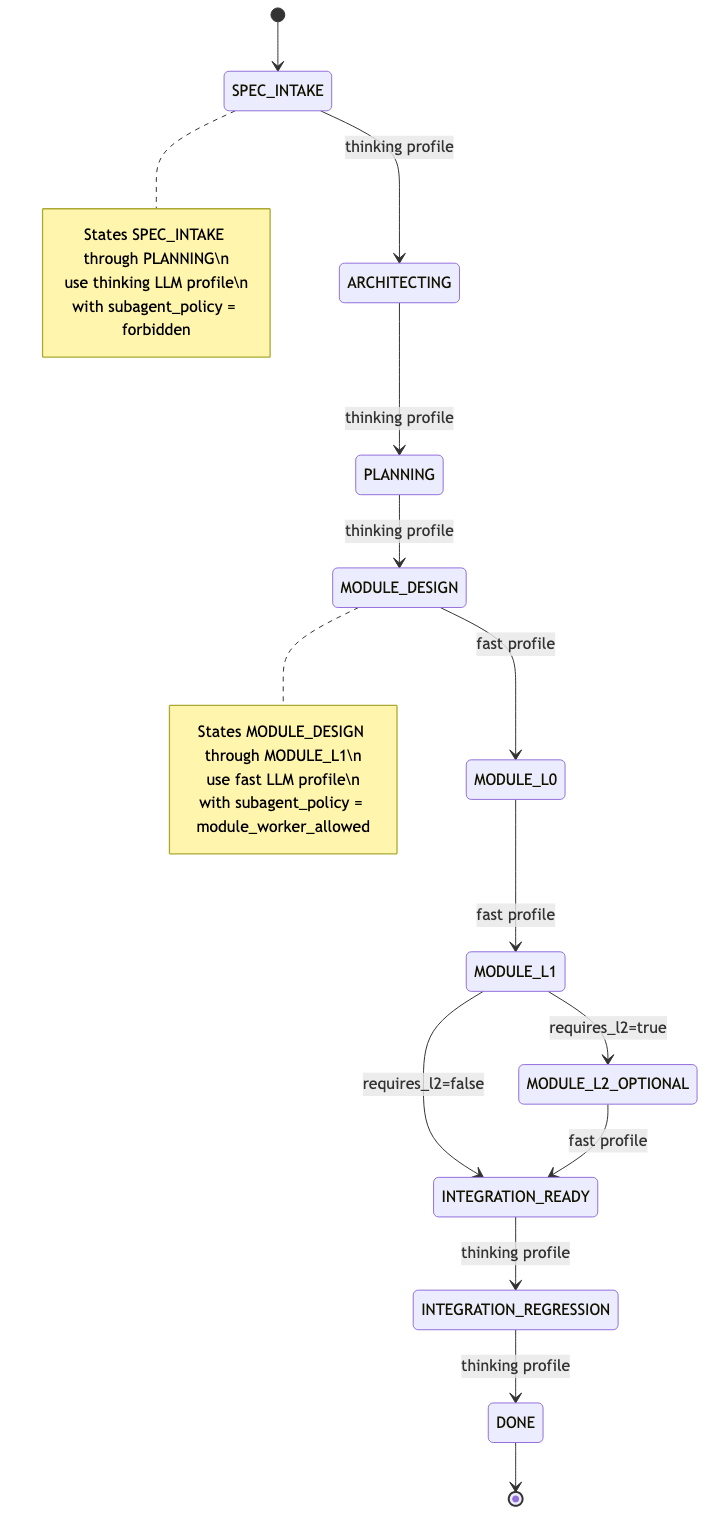
\includegraphics[keepaspectratio,alt={图 4-1: 编排器10状态转移图}]{../fpga_flow/diagrams/14_orchestrator_states.png}}
\caption{图 4-1: 编排器10状态转移图}
\end{figure}

\subsubsection{4.1.2
状态转移逻辑}\label{ux72b6ux6001ux8f6cux79fbux903bux8f91}

\texttt{AESWorkflowOrchestrator.next\_state\_after\_success()}
方法封装了所有成功路径的状态转移逻辑，其转移字典如下：

\begin{verbatim}
SPEC_INTAKE     → ARCHITECTING
ARCHITECTING    → PLANNING
PLANNING        → MODULE_DESIGN
MODULE_DESIGN   → MODULE_L0
MODULE_L0       → MODULE_L1
MODULE_L1       → MODULE_L2_OPTIONAL（当 requires_l2=True）
              → INTEGRATION_READY  （当 requires_l2=False）
MODULE_L2_OPTIONAL → INTEGRATION_READY
INTEGRATION_READY  → INTEGRATION_REGRESSION
INTEGRATION_REGRESSION → DONE
\end{verbatim}

\texttt{requires\_l2} 参数由节点的 \texttt{l2\_policy}
字段决定：\texttt{l2\_policy=\textquotesingle{}skip\textquotesingle{}}
时为
\texttt{False}，其他情况（\texttt{conditional}、\texttt{required}）为
\texttt{True}。\texttt{describe\_state\_progression()}
方法提供完整的状态链追踪，返回包含每个状态的 \texttt{StateTraceEntry}
列表，便于调试和日志记录。

\textbf{表 4-1: 每个状态的语义、执行者、输入/输出}

{\def\LTcaptype{none} % do not increment counter
\begin{longtable}[]{@{}
  >{\raggedright\arraybackslash}p{(\linewidth - 8\tabcolsep) * \real{0.1538}}
  >{\raggedright\arraybackslash}p{(\linewidth - 8\tabcolsep) * \real{0.1538}}
  >{\raggedright\arraybackslash}p{(\linewidth - 8\tabcolsep) * \real{0.2308}}
  >{\raggedright\arraybackslash}p{(\linewidth - 8\tabcolsep) * \real{0.2308}}
  >{\raggedright\arraybackslash}p{(\linewidth - 8\tabcolsep) * \real{0.2308}}@{}}
\toprule\noalign{}
\begin{minipage}[b]{\linewidth}\raggedright
状态
\end{minipage} & \begin{minipage}[b]{\linewidth}\raggedright
语义
\end{minipage} & \begin{minipage}[b]{\linewidth}\raggedright
执行主体
\end{minipage} & \begin{minipage}[b]{\linewidth}\raggedright
主要输入
\end{minipage} & \begin{minipage}[b]{\linewidth}\raggedright
主要输出
\end{minipage} \\
\midrule\noalign{}
\endhead
\bottomrule\noalign{}
\endlastfoot
SPEC\_INTAKE & 规格摄入与验证 & 框架合成层 & 系统目标字符串 & SpecIR \\
ARCHITECTING & DAG 结构生成 & 框架合成层 & SpecIR & PlanDAG \\
PLANNING & 集成清单生成 & 框架合成层 & SpecIR + PlanDAG &
IntegrationManifest \\
MODULE\_DESIGN & 工作区初始化与 Memory 预填充 & 框架 + Module Worker &
PlanDAGNode & 草稿 RTL/TB + 合约 JSON \\
MODULE\_L0 & 编译门控 & 框架 L0Executor & 草稿 RTL 文件 & compile.log +
编译结果 JSON \\
MODULE\_L1 & 仿真 + Checkpoint 验证 & 框架 L1Executor & 草稿 RTL + TB &
simulation.log + Checkpoint 汇总 \\
MODULE\_L2\_OPTIONAL & 鲁棒性随机测试 & 框架 L2CampaignExecutor + L2
Campaign Agent & 晋升 RTL + 向量集 & fragility\_summary.json +
counterexample.json \\
INTEGRATION\_READY & 依赖闭包验证 & 框架合成层 & 全部 PROMOTED 记录 &
集成顶层节点选择 \\
INTEGRATION\_REGRESSION & 三种集成 campaign & 框架
IntegrationRegressionExecutor & 集成清单 + 晋升 RTL & 三种 campaign
Checkpoint 结果 \\
DONE & 终态汇总 & Finalizer Orchestrator & 所有 artifact 路径 &
终态报告 \\
\end{longtable}
}

\begin{center}\rule{0.5\linewidth}{0.5pt}\end{center}

\subsection{4.2 AgentExecutionPolicy
策略分层}\label{agentexecutionpolicy-ux7b56ux7565ux5206ux5c42}

AgentExecutionPolicy 的设计是领域无关的------它将状态映射到 LLM Profile
和子代理策略，这一映射机制适用于任何硬件设计自动化场景。具体的映射内容基于通用的任务复杂度分析：跨模块决策需要深度推理，节点本地执行需要快速响应。

\subsubsection{4.2.1
策略模型设计}\label{ux7b56ux7565ux6a21ux578bux8bbeux8ba1}

\texttt{AgentExecutionPolicy} 是一个 Pydantic 模型（同样使用
\texttt{extra=\textquotesingle{}forbid\textquotesingle{}}），包含三个核心字段：

\begin{itemize}
\tightlist
\item
  \texttt{state\_profiles:\ dict{[}OrchestratorState,\ LLMProfileName{]}}：状态到
  LLM Profile 的映射
\item
  \texttt{state\_subagents:\ dict{[}OrchestratorState,\ SubagentPolicy{]}}：状态到子代理策略的映射
\item
  \texttt{repair\_attempt\_threshold:\ int}：修复升级阈值（默认 2，下限
  1）
\end{itemize}

\texttt{@model\_validator} 强制要求 \texttt{state\_profiles} 和
\texttt{state\_subagents} 必须覆盖全部 9 个活跃状态（\texttt{DONE}
状态不需要策略映射，因为它是终态）。这一完整性检查意味着系统永远不会出现''进入某个状态但找不到对应策略''的情况------若在系统初始化时发现缺失映射，将立即抛出
\texttt{ValueError} 阻止系统启动。

\subsubsection{4.2.2
完整策略映射表}\label{ux5b8cux6574ux7b56ux7565ux6620ux5c04ux8868}

\textbf{表 4-2: OrchestratorState → Policy 完整映射表}

{\def\LTcaptype{none} % do not increment counter
\begin{longtable}[]{@{}
  >{\raggedright\arraybackslash}p{(\linewidth - 6\tabcolsep) * \real{0.1622}}
  >{\raggedright\arraybackslash}p{(\linewidth - 6\tabcolsep) * \real{0.3243}}
  >{\raggedright\arraybackslash}p{(\linewidth - 6\tabcolsep) * \real{0.2703}}
  >{\raggedright\arraybackslash}p{(\linewidth - 6\tabcolsep) * \real{0.2432}}@{}}
\toprule\noalign{}
\begin{minipage}[b]{\linewidth}\raggedright
状态
\end{minipage} & \begin{minipage}[b]{\linewidth}\raggedright
LLM Profile
\end{minipage} & \begin{minipage}[b]{\linewidth}\raggedright
子代理策略
\end{minipage} & \begin{minipage}[b]{\linewidth}\raggedright
设计意图
\end{minipage} \\
\midrule\noalign{}
\endhead
\bottomrule\noalign{}
\endlastfoot
SPEC\_INTAKE & THINKING & FORBIDDEN & 规格验证需要精确推理，禁止委派 \\
ARCHITECTING & THINKING & FORBIDDEN & DAG 生成是框架操作，无 LLM 委派 \\
PLANNING & THINKING & FORBIDDEN & 集成清单生成，无子代理 \\
MODULE\_DESIGN & FAST & MODULE\_WORKER\_ALLOWED &
工作区初始化委派给节点工作者 \\
MODULE\_L0 & FAST & MODULE\_WORKER\_ALLOWED &
编译门控可委派给节点工作者 \\
MODULE\_L1 & FAST & MODULE\_WORKER\_ALLOWED &
仿真验证可委派给节点工作者 \\
MODULE\_L2\_OPTIONAL & FAST & L2\_CAMPAIGN\_ALLOWED & L2
测试专用子代理 \\
INTEGRATION\_READY & THINKING & FORBIDDEN & 集成就绪判断是框架操作 \\
INTEGRATION\_REGRESSION & THINKING & FORBIDDEN &
集成回归由思考型编排器独占 \\
\end{longtable}
}

\subsubsection{4.2.3 LLM Profile
分级的设计依据}\label{llm-profile-ux5206ux7ea7ux7684ux8bbeux8ba1ux4f9dux636e}

\texttt{LLMProfileName}
枚举定义了两个值：\texttt{DEEPSEEK\_OFFICIAL\_THINKING} 和
\texttt{DEEPSEEK\_OFFICIAL\_FAST}，分别对应深度思考模式和快速执行模式。

\textbf{使用思考模式（THINKING）的状态}：\texttt{SPEC\_INTAKE}、\texttt{ARCHITECTING}、\texttt{PLANNING}、\texttt{INTEGRATION\_READY}、\texttt{INTEGRATION\_REGRESSION}。这些状态涉及跨模块推理（如判断
4
个模块的接口是否一致）、工作流级别的决策（如决定是否触发升级）或需要精确分析集成测试失败原因。思考模式的
\texttt{reasoning\_effort=\textquotesingle{}medium\textquotesingle{}} 使
LLM
进行内部推理链（Chain-of-Thought），提升复杂推理的可靠性，但会增加延迟和
API 成本。

\textbf{使用快速模式（FAST）的状态}：\texttt{MODULE\_DESIGN}、\texttt{MODULE\_L0}、\texttt{MODULE\_L1}、\texttt{MODULE\_L2\_OPTIONAL}。这些状态的任务高度局部化------每个
Module Worker 只需要处理一个模块的代码，参考实现已通过 Memory
预填充，任务边界清晰。快速模式的
\texttt{reasoning\_effort=\textquotesingle{}none\textquotesingle{}}
跳过内部推理步骤，直接生成输出，响应时间显著降低。

\subsubsection{4.2.4 SubagentPolicy
三级控制}\label{subagentpolicy-ux4e09ux7ea7ux63a7ux5236}

\texttt{SubagentPolicy} 枚举定义了三个级别的子代理委派控制：

\textbf{FORBIDDEN（禁止委派）}：编排器不得在当前状态下启动子代理。适用于需要编排器独占控制的阶段：规格/架构/规划（这三个阶段由框架合成层执行，LLM
参与度低，不需要子代理）以及集成就绪/集成回归（这两个阶段需要跨模块推理，委派给子代理会导致上下文分散）。

\textbf{MODULE\_WORKER\_ALLOWED（允许模块工作者）}：编排器可以将节点本地任务委派给
Module Worker 子代理。Module Worker
的作用域严格限定：\texttt{build\_module\_worker\_spec()} 返回的
\texttt{AgentSpawnSpec} 中，\texttt{writable\_paths} 仅包含该节点的 RTL
文件和测试台文件，\texttt{allowed\_states} 仅包含
\texttt{MODULE\_DESIGN}/\texttt{MODULE\_L0}/\texttt{MODULE\_L1}
三个状态。这一双重约束（路径约束 + 状态约束）确保 Module Worker
无法越权修改其他模块的代码或执行集成级别的操作。

\textbf{L2\_CAMPAIGN\_ALLOWED（允许 L2 测试代理）}：编排器可以启动专用的
L2 测试活动子代理。L2 Campaign Agent 的
\texttt{build\_l2\_campaign\_spec()} 确保测试代理不持有 RTL/TB
可写路径，且持有的 \texttt{run\_executor} 工具在 L2
阶段不允许触发代码编辑操作。

\begin{figure}
\centering
\pandocbounded{
\includegraphics[keepaspectratio,alt={图 4-2: SDK Agent层级结构}]{../fpga_flow/diagrams/05_sdk_agent_hierarchy.png}}
\caption{图 4-2: SDK Agent层级结构}
\end{figure}

\begin{center}\rule{0.5\linewidth}{0.5pt}\end{center}

\subsection{4.3
升级策略设计}\label{ux5347ux7ea7ux7b56ux7565ux8bbeux8ba1}

\subsubsection{4.3.1
升级触发条件}\label{ux5347ux7ea7ux89e6ux53d1ux6761ux4ef6}

\texttt{AgentExecutionPolicy.should\_escalate()}
是系统中唯一的升级决策函数，其签名为：

\begin{Shaded}
\begin{Highlighting}[]
\KeywordTok{def}\NormalTok{ should\_escalate(}
    \VariableTok{self}\NormalTok{,}
\NormalTok{    repair\_attempts: }\BuiltInTok{int}\NormalTok{,}
    \OperatorTok{*}\NormalTok{,}
\NormalTok{    cross\_module\_issue: }\BuiltInTok{bool} \OperatorTok{=} \VariableTok{False}\NormalTok{,}
\NormalTok{    state\_machine\_issue: }\BuiltInTok{bool} \OperatorTok{=} \VariableTok{False}\NormalTok{,}
\NormalTok{    interface\_issue: }\BuiltInTok{bool} \OperatorTok{=} \VariableTok{False}\NormalTok{,}
\NormalTok{) }\OperatorTok{{-}\textgreater{}} \BuiltInTok{bool}\NormalTok{:}
    \ControlFlowTok{return}\NormalTok{ (}
\NormalTok{        repair\_attempts }\OperatorTok{\textgreater{}=} \VariableTok{self}\NormalTok{.repair\_attempt\_threshold}
        \KeywordTok{or}\NormalTok{ cross\_module\_issue}
        \KeywordTok{or}\NormalTok{ state\_machine\_issue}
        \KeywordTok{or}\NormalTok{ interface\_issue}
\NormalTok{    )}
\end{Highlighting}
\end{Shaded}

该函数的逻辑体现了两类不同性质的升级触发场景：

\textbf{数量触发}：当
\texttt{repair\_attempts\ \textgreater{}=\ repair\_attempt\_threshold}
时，说明 Module Worker
在有限次数内未能修复问题，继续让其尝试的边际收益递减。\texttt{repair\_attempt\_threshold}
默认为 2，即 Module Worker 最多允许两轮修复尝试。

\textbf{性质触发}：当
\texttt{cross\_module\_issue=True}（问题跨越模块边界，如接口信号宽度不匹配）、\texttt{state\_machine\_issue=True}（涉及
FSM 逻辑错误，如状态转移条件错误）或
\texttt{interface\_issue=True}（端口名称或方向不一致）时，无论已进行多少次修复，均立即升级。这三类问题的共同特征是：它们不能被节点本地的
Module Worker 独立解决，必须由具有全局视野的思考型编排器介入。

\subsubsection{4.3.2
修复预算管理}\label{ux4feeux590dux9884ux7b97ux7ba1ux7406}

\texttt{generation.py} 中的 \texttt{repair\_budget\_for\_node()}
函数根据节点的 \texttt{integration\_role} 字段分配差异化的修复预算：

\begin{Shaded}
\begin{Highlighting}[]
\KeywordTok{def}\NormalTok{ repair\_budget\_for\_node(node: PlanDAGNode) }\OperatorTok{{-}\textgreater{}} \BuiltInTok{int}\NormalTok{:}
    \ControlFlowTok{if}\NormalTok{ node.integration\_role }\KeywordTok{in}\NormalTok{ (}\StringTok{\textquotesingle{}top\textquotesingle{}}\NormalTok{, }\StringTok{\textquotesingle{}sink\textquotesingle{}}\NormalTok{):}
        \ControlFlowTok{return}\NormalTok{ TOP\_MODULE\_REPAIR\_BUDGET  }\CommentTok{\# = 3}
    \ControlFlowTok{return}\NormalTok{ DEFAULT\_REPAIR\_BUDGET  }\CommentTok{\# = 2}
\end{Highlighting}
\end{Shaded}

顶层/sink
节点（\texttt{aes128\_encrypt\_core}，\texttt{integration\_role=\textquotesingle{}sink\textquotesingle{}}）获得
3 次修复机会，其他节点（叶节点和支撑节点）获得 2
次机会。这一差异化预算设计的依据是：顶层加密核心是整个系统最复杂的模块，其
FSM 逻辑（\texttt{IDLE}→\texttt{ROUND}→\texttt{DONE}
三状态）涉及多个子模块的集成，修复时更容易需要多轮迭代。相比之下，\texttt{aes\_sbox}
等叶节点逻辑简单，若 2 次修复后仍失败，说明问题已超出 Module Worker
的能力范围，升级至编排器处理更为合适。

这一有限预算机制与基于AutoGen的线性pipeline方案中 Debug Agent
的无限重试策略形成鲜明对比：无限重试在理论上提供了更多自我修复机会，但在实践中可能导致系统陷入无效循环（例如
Agent 每次修复都破坏了其他已通过的
Checkpoint），且没有收敛保证。有限预算确保了系统的终止性。

\subsubsection{4.3.3
升级后的行为}\label{ux5347ux7ea7ux540eux7684ux884cux4e3a}

升级发生后，框架将失败模块的完整上下文（\texttt{RepairContract}、验证日志路径、已尝试的修复历史）附加到编排器会话的下一条消息中。思考型编排器在接收到升级信息后，可以采取以下几种策略之一：

\begin{itemize}
\tightlist
\item
  重新分析错误，生成新的 \texttt{RepairContract} 并重置修复计数
\item
  判断该模块为不可修复（\texttt{BLOCKED}
  状态），记录失败并继续处理其他节点
\item
  判断问题为跨模块接口不兼容，触发对相关模块的联合修复
\end{itemize}

\begin{figure}
\centering
\pandocbounded{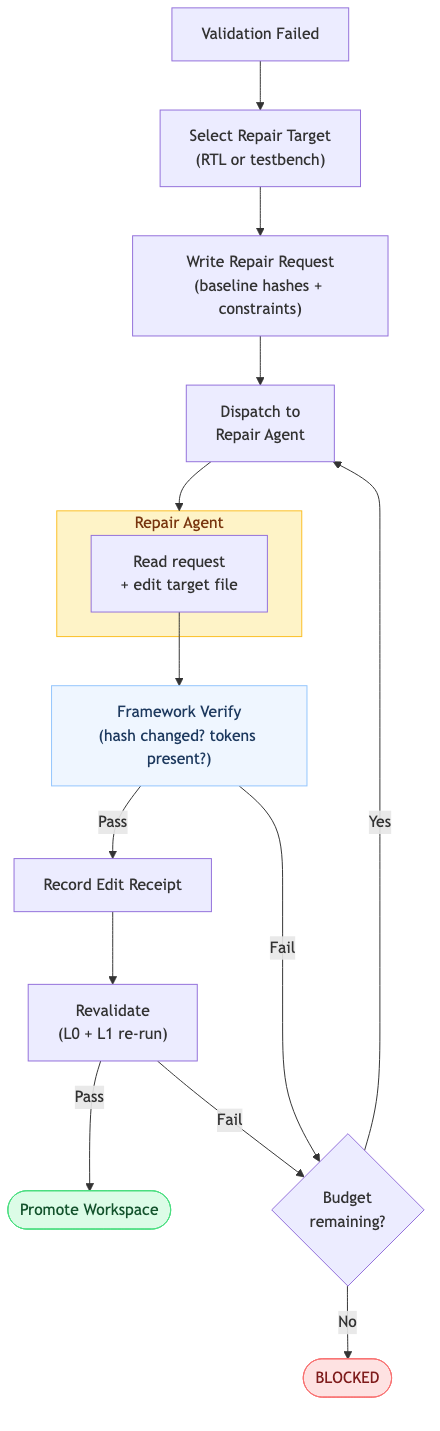
\includegraphics[keepaspectratio,alt={图 4-3: 修复循环流程}]{../fpga_flow/diagrams/06_repair_cycle.png}}
\caption{图 4-3: 修复循环流程}
\end{figure}

\begin{center}\rule{0.5\linewidth}{0.5pt}\end{center}

\subsection{4.4 框架控制 vs Agent
控制}\label{ux6846ux67b6ux63a7ux5236-vs-agent-ux63a7ux5236}

\subsubsection{4.4.1
核心设计决策}\label{ux6838ux5fc3ux8bbeux8ba1ux51b3ux7b56}

框架控制与 Agent
控制的对比分析适用于所有多智能体硬件设计自动化场景，不限于 AES-128
案例。LLM
在控制流中的典型失败模式（提前宣告成功、无限修复循环、范围漂移）是所有
LLM 驱动的工程自动化系统面临的共性挑战。

``为什么不让 LLM
决定何时推进工作流状态？''这一问题是本框架最核心的设计决策点。理解这一决策需要首先分析
LLM 在控制流场景中的典型失败模式。

\textbf{失败模式一：提前宣告成功（幻觉）}。LLM
在生成响应时可能基于局部信息做出乐观判断------例如，仿真输出中出现了''PASS''字样（但这是某个非必需
Checkpoint 的 PASS），LLM
便宣告该模块已通过验证，触发晋升操作。实际上，\texttt{CHK\_CIPHERTEXT\_MATCH}
这一关键 Checkpoint 从未出现在日志中。在 Prompt-controlled
方案中，这类幻觉式提前完成极难通过提示词工程杜绝；在本框架中，由于
Checkpoint 汇总由 \texttt{summarize\_required\_checkpoints()}
机器执行，LLM 的任何''宣告''都不会影响工作区状态的实际转变。

\textbf{失败模式二：无限修复循环}。LLM
在修复代码时可能反复修改同一段逻辑，每次修改都基于对错误的不同解读，但始终无法触达根本原因。没有外部预算限制的情况下，这种行为可以持续很长时间，消耗大量
API 调用和等待时间。本框架通过 \texttt{repair\_attempt\_threshold}
硬性终止修复循环，确保系统不会无限等待 LLM 的自我修复收敛。

\textbf{失败模式三：范围漂移（Scope Drift）}。LLM
在修复某个模块时可能''顺手''修改了其他模块的接口定义，以期解决接口不一致问题。这种越界修改在当时可能让测试通过，但破坏了系统的其他部分。\texttt{WORKER\_LOCAL\_SCOPE}
阶段混入约束从提示词层面限制 Agent
的行为范围，但更根本的保护来自框架层面的可写路径约束------\texttt{build\_module\_worker\_spec(node)}
生成的 \texttt{AgentSpawnSpec} 中，\texttt{writable\_paths}
仅包含该节点的文件，OpenHands SDK 在底层强制执行此约束。

\subsubsection{4.4.2 FRAMEWORK\_OWNS\_PROGRESS\_CONTRACT
的设计意图}\label{framework_owns_progress_contract-ux7684ux8bbeux8ba1ux610fux56fe}

\texttt{prompt\_contracts.py} 中的
\texttt{FRAMEWORK\_OWNS\_PROGRESS\_CONTRACT} 是一个
\texttt{BaseContract}，包含以下约束行：

\begin{verbatim}
The framework, not you, owns batch progression and workflow completion.
\end{verbatim}

这条约束被注入所有 Agent 角色的系统提示词，配合
\texttt{ORCHESTRATOR\_NO\_FINISH}
阶段混入（\texttt{Do\ not\ call\ finish\ in\ the\ execution\ conversation.}）和
\texttt{ORCHESTRATOR\_ONLY\_CURRENT\_BATCH}
阶段混入（\texttt{Execute\ only\ the\ current\ batch\ handed\ to\ this\ conversation.\ Do\ not\ infer\ future\ batches,\ merge\ batches,\ or\ summarize\ the\ whole\ workflow\ as\ complete.}），构建了三重语义锁定：

\begin{enumerate}
\def\labelenumi{\arabic{enumi}.}
\tightlist
\item
  \textbf{控制权归属声明}：明确告知 Agent 它不拥有工作流推进的控制权
\item
  \textbf{行动禁止规则}：禁止执行编排器调用 \texttt{finish()}
\item
  \textbf{批次边界约束}：禁止 Agent 基于推断跨越批次边界
\end{enumerate}

三重约束共同作用，确保即使在 LLM
产生错误乐观判断时，其输出也不会导致工作流状态的错误推进。

\subsubsection{4.4.3 Batch Gate
回调模式}\label{batch-gate-ux56deux8c03ux6a21ux5f0f}

\texttt{ConversationRunner.run\_current\_batch\_until\_gate()} 实现了
Batch Gate（批次门控）模式，这是框架控制架构的运行时实现：

\begin{Shaded}
\begin{Highlighting}[]
\KeywordTok{def}\NormalTok{ run\_current\_batch\_until\_gate(}
    \VariableTok{self}\NormalTok{,}
\NormalTok{    conversation,}
\NormalTok{    message: }\BuiltInTok{str}\NormalTok{,}
    \OperatorTok{*}\NormalTok{,}
\NormalTok{    batch\_gate: Callable[[], }\BuiltInTok{bool}\NormalTok{],}
\NormalTok{    timeout\_s: }\BuiltInTok{float} \OperatorTok{=} \FloatTok{180.0}\NormalTok{,}
\NormalTok{    poll\_interval\_s: }\BuiltInTok{float} \OperatorTok{=} \FloatTok{0.2}\NormalTok{,}
\NormalTok{) }\OperatorTok{{-}\textgreater{}}\NormalTok{ BatchRunSummary:}
\end{Highlighting}
\end{Shaded}

该方法的工作机制如下： 1. 向 Agent
会话发送当前批次任务消息，在独立线程中启动 Agent 对话循环 2. 主线程以
0.2 秒间隔轮询 \texttt{batch\_gate()} 回调（该回调检查文件系统中的
artifact 是否满足批次完成条件） 3. 当 \texttt{batch\_gate()} 返回
\texttt{True} 时，立即调用 \texttt{conversation.pause()} 暂停 Agent
会话，不等待 Agent 自行结束 4. 若超过 \texttt{timeout\_s}
秒后门控仍未满足，强制暂停会话并记录超时状态

这一模式的关键特征是：\textbf{文件系统是 Agent
与框架之间的唯一通信通道}。Agent 通过写文件（生成
RTL、写出编辑收据、输出验证报告）向框架传递工作进度；框架通过读文件（检查
\texttt{NodeWorkspaceRecord} 状态、解析 \texttt{EditReceipt}、校验
Checkpoint 汇总）判断批次是否完成。这种设计有两个重要优点：一是 Agent
的任何言辞性声明（``我已完成此模块''）不产生任何框架层面的效果；二是文件系统的持久性使得即使
Agent 会话意外终止，框架也能从 artifact 文件中恢复工作状态。

\begin{figure}
\centering
\pandocbounded{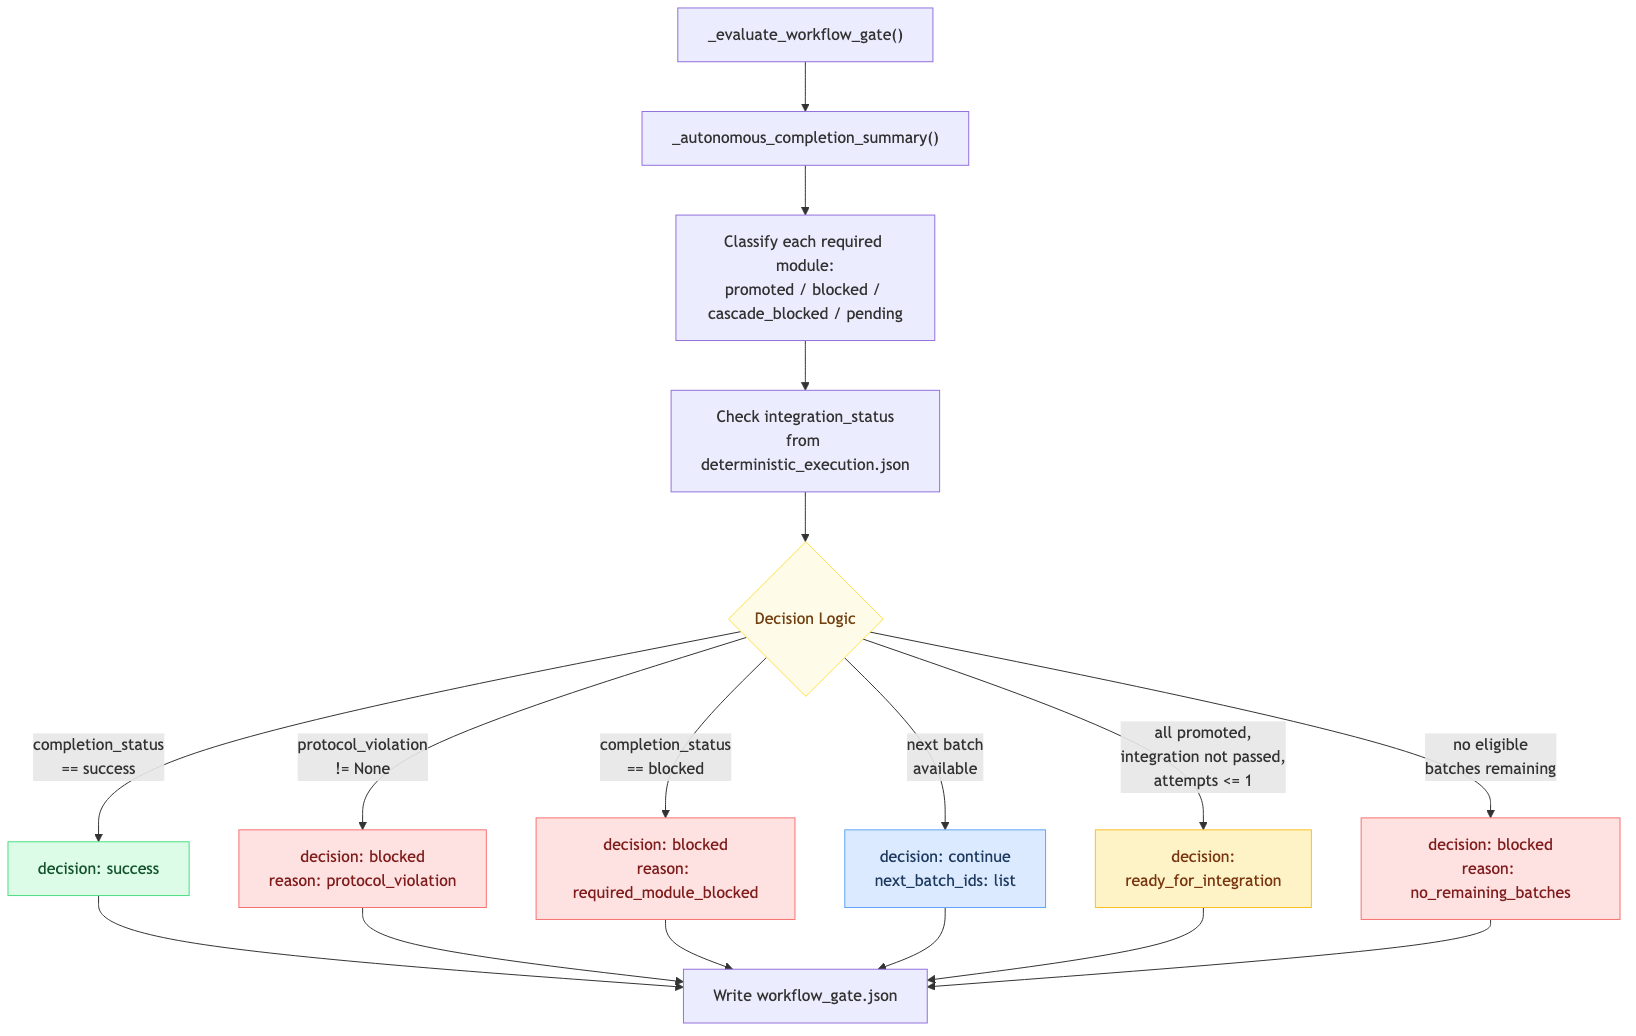
\includegraphics[keepaspectratio,alt={图 4-4: 工作流门控机制}]{../fpga_flow/diagrams/09_workflow_gate.png}}
\caption{图 4-4: 工作流门控机制}
\end{figure}

\subsubsection{4.4.4 与 AutoGen
方案的对比分析}\label{ux4e0e-autogen-ux65b9ux6848ux7684ux5bf9ux6bd4ux5206ux6790}

AutoGen 方案采用 AutoGen 的 \texttt{human\_input\_mode="NEVER"} 配置，使
Agent 链在无人工干预的情况下自主运行至完成。这一配置的含义是：AutoGen
的每个 Agent
在完成自己的任务后，自主决定是否结束对话或将控制权传递给下一个
Agent。控制流本质上由 LLM 的输出决定------当 Agent
输出''TERMINATE''关键词时，对话结束。

这种方式的主要风险在于：控制流的可靠性完全依赖 LLM
在正确时机输出正确关键词。若 LLM
错误地在验证尚未完成时输出''TERMINATE''，整个工作流便提前结束；若 LLM
陷入循环而不输出终止信号，工作流便永不结束。缺乏外部检查点（Checkpoint）意味着工作流的中间状态完全不透明。

本框架通过状态机 + Batch Gate +
\texttt{FRAMEWORK\_OWNS\_PROGRESS\_CONTRACT}
三层机制，将控制流的可靠性从''依赖 LLM
的正确输出''提升到''依赖框架代码的正确执行''。这一转变使系统的可靠性具备了数学可验证性：只要框架代码（Python
+ Pydantic）正确，批次推进决策就不会受到 LLM 幻觉的干扰。

\begin{center}\rule{0.5\linewidth}{0.5pt}\end{center}

\subsection{4.5 小结}\label{ux5c0fux7ed3}

本章深入分析了系统的 10 状态编排状态机与 \texttt{AgentExecutionPolicy}
策略分层机制。核心设计理念可归纳为三点：

\textbf{第一，状态语义精确化}。10 个状态不仅是阶段标记，更是 LLM Profile
选择和子代理委派策略的索引键，每个状态的语义与其对应的策略绑定。\texttt{AgentExecutionPolicy}
的完整性验证确保策略映射在系统初始化时即经过检查，而非在运行时动态推断。

\textbf{第二，策略分层精准化}。THINKING/FAST 双 Profile
的分配规则是：跨模块推理用 THINKING，节点本地执行用
FAST。FORBIDDEN/MODULE\_WORKER\_ALLOWED/L2\_CAMPAIGN\_ALLOWED
三级子代理策略的分配规则是：需要全局视野的阶段禁止委派，需要并行执行的节点本地任务允许委派给专用子代理。

\textbf{第三，控制权内聚于框架}。通过
\texttt{FRAMEWORK\_OWNS\_PROGRESS\_CONTRACT}、\texttt{ORCHESTRATOR\_NO\_FINISH}、\texttt{batch\_gate}
回调和有限修复预算四层机制，系统确保了工作流推进决策始终由可验证的框架代码而非不可靠的
LLM 输出驱动。这是本框架区别于传统 Prompt-controlled
多智能体方案的根本性架构差异，也是系统在面对 LLM
幻觉和不可靠性时保持工作流正确性的核心保障。

本章阐述的编排状态机与策略分层机制在架构层面是通用的：状态语义、策略映射和控制权分配原则均不依赖于特定的硬件设计对象。AES-128
验证案例中的具体实例化内容是案例相关的，但框架的状态机骨架和策略分层逻辑可直接复用于其他
DAG 可分解的多模块设计。
